\cleardoublepage
\chapter{Theorie}
\label{theory}

Dieses Kapitel soll einen Überblick über die zu simulierenden Prozesse und benutzten Simulationsmethoden geben.
Dazu stellt Abschnitt \ref{depositions} die Prinzipien der drei Arten der Gasphasenabscheidungen vor, Abschnitte \ref{md} und \ref{kmc} behandeln jeweils die Simulationsmethoden der Molekulardynamik und Kinetischen Monte-Carlo-Simulationen.
Zuletzt geht Abschnitt \ref{datastructures} auf die verschiedenen Datenstrukturen ein, die genutzt werden, um effiziente Simulationen großer Simulationsräume zu ermöglichen.

\section{Gasphasenabscheidungen}

Gasphasenabscheidungen sind eine Klasse von Verfahren, bei denen dünne Schichten durch physikalische oder chemische Prozesse aus der Gasphase auf eine Oberfläche aufgetragen werden.
Sie teilen sich in \textbf{Physikalische Gasphasenabscheidung} (PVD, Physical Vapor Deposition), \textbf{Chemische Gasphasenabscheidung} (CVD, Chemical Vapor Deposition) und \textbf{Atomlagenabscheidung} (ALD, Atomic Layer Deposition) auf, die im folgenden betrachtet werden.

Ihnen ist allgemein, dass einzelne Atome oder Moleküle auf der Oberfläche aufkommen, dort physikalisch oder chemisch adsorbiert werden und eventuelle Nebenprodukte aus dem Reaktor gespült werden, wodurch mit vorhersehbarer Rate eine dünne Schicht des Zielmateriales aufwächst.
Tabellen \ref{tab:deposition-comparison} und \ref{tab:deposition-materials} stellen jeweils Charakteristiken und mögliche Materialien für die drei Prozesse dar.

\missingfigure{Reaktoren}

\begin{table}
  \centering
  \begin{tabularx}{\textwidth}{|X|ccc|}
    \hline
    Prozesscharakteristiken & \textbf{PVD} & \textbf{CVD} & \textbf{ALD} \\
    \hline
    reaktiv &  & \cmark & \cmark \\
    kontinuierlich & \cmark & \cmark & zyklisch \\
    Gas-Edukte & Atome, Moleküle & Precursor-Moleküle & Precursor-Moleküle \\
    \# Edukte & 1 & 1+ & 2+ \\
    Nebenprodukte & & \cmark & \cmark \\
    Wachstumsrate & $\sim t$ & $\sim t$ & $\sim n_\text{cyc.}$ \\
    \hline
  \end{tabularx}
  \caption[Prozesscharakteristiken der Abscheidungsarten]{Vergleich der Abscheidungsarten}
  \label{tab:deposition-comparison}
\end{table}

\begin{table}
  \centering
  \begin{tabularx}{\textwidth}{XXXXXXXXX}
    & \angled{Metalle} & \angled{Legierungen} & \angled{Metalloxide} & \angled{Nitride} & \angled{Chloride} & \angled{Silizium}  & \angled{Siliziumoxid} & \angled{Diamant} \\
    \hline
    \textbf{PVD} &\cmark&\cmark&&&&\cmark&&?\\
    \textbf{CVD} &\cmark&?&\cmark&\cmark&\cmark&\cmark&?&?\\
    \textbf{ALD} &\cmark&?&\cmark&\cmark&\cmark&\cmark&\cmark&\cmark\\
  \end{tabularx}
  \caption[Mögliche Produkte der Abscheidungsarten]{Mögliche Produkte der Abscheidungsarten. Weitergehende Informationen finden sich in der Literatur für PVD\cite{asd}, CVD\cite{asd} und ALD\cite{puurunen_surface_2005}.}
  \todo[inline]{Referenzen für abgeschiedene Systeme}
  \label{tab:deposition-materials}
\end{table}

\subsection{Physikalische Gasphasenabscheidung}

PVD ist kontinuierlich und nicht reaktiv, arbeitet also mit Atomen oder Molekülen, die physikalisch auf der Oberfläche adsorbieren.
Beispielsweise werden beim Sputtering durch energiereiche Partikel (Argon-Plasma) einzelne Atome aus dem sogenannten Target geschlagen, die dann auf dem Substrat eine homogene, dünne Schicht bilden.
Durch die Nutzung mehrerer Targets (Cosputtering) oder mehrerer Atomsorten in einem Target lassen sich auch Legierungen und andere mehrelementige Materialien abscheiden.
\todo{Referenzen für alles}

\subsection{Chemische Gasphasenabscheidung}

CVD wächst durch chemische Adsorption eines oder mehrerer Precursor-Moleküles eine dünne Schicht auf dem Substrat auf.
Dazu werden die Precursorgase zeitgleich in den Reaktor geleitet, wo sie über die Substratoberfläche strömen und Reaktionen ermöglichen.
Die dabei entstehenden Nebenprodukte werden mit dem Gasstrom aus dem Reaktor geführt, um die aufwachsende Schicht nicht zu verunreinigen.
\todo{zu abrupter Übergang}

Passende Precursor-Kombinationen zu finden, gestaltet sich oft schwierig, da sie idealerweise erst auf der Oberfläche und nicht in der Gasphase reagieren und dabei inerte Nebenprodukte erzeugen sollen.
Weitere Kriterien wie Prozesstemperaturen, Energiebarrieren und komplizierte Reaktionspfade erschweren die Suche zusätzlich.
Im Gegensatz zu PVD kann CVD dafür auf allen Substraten, über deren Oberfläche ein kontinuierlicher Gasfluss möglich ist, eine dünne Schicht abscheiden.
Dies beinhaltet Stufen, Rillen und anderweitig strukturierte Substrate ebenso wie Poren durch das Substrat.

\subsection{Atomlagenabscheidung}

ALD entstand als Abwandlung der CVD, bei der zwei Precursorgase wechselweise in den Reaktor geleitet werden.
So werden einerseits Gasphasenreaktionen vermieden, andererseits wächst die Schicht nicht mehr kontinuierlich, sondern zyklisch mit einer Höhe pro Zyklus (GPC, Growth per Cycle), die von der Wahl des Precursorpaares abhängt.

\begin{figure}
  \def\svgwidth{\textwidth}
  \input{img/ald-schema.pdf_tex}
  \caption[ALD-Schema]{ALD-Schema: dsa ald}
  \label{fig:ald-schema}
\end{figure}

\clearpage
\section{Molekulardynamik}
\label{md}

Ursprünglich mit dem Ziel der klassischen Simulation idealer Gase entwickelt, wurde die Molekulardynamik seither um die Fähigkeit zur Simulation von Festkörpern, organischen Molekülen und Reaktionen erweitert.
Dadurch findet sie Anwendung in Simulationen von Materialien und chemischen Stoffen bei beliebigen Temperaturen und Drücken, um deren Verhalten vorhersagen und auf reale Prozesse zurückführen zu können.

Nachfolgend möchte ich einen kurzen Überblick über die Formulierung molekulardynamischer Methoden geben (Abschnitt \ref{mdformulation}) und im Anschluss auf die Unterschiede und Möglichkeiten der Kraftfelder eingehen (Abschnitt \ref{mdforcefields}).

\subsection{Formulierung}
\label{mdformulation}

Molekulardynamik ist eine klassische Vielteilchenmethode, die jedem Teilchen des Systemes \todo{wieso $R$?}$R$ eine Masse $m$, eine Position $\vec r$, einen Impuls $\vec p$ und Kräfte entsprechend eines lokalen Kraftfeldes $\vec{F}(R)$ oder eventuellen Randbedingungen zuweist.
Entsprechend der Born-Oppenheimer-Näherung, nach der die Elektronen eines chemischen Systemes an ihre Atomkerne gebunden sind und schnell genug auf Änderungen des Systemes reagieren, genügt es, die Atome als Punktmassen an der Position ihres Atomkernes zu betrachten.
Elektronische und sonstige Interaktionen werden dann durch die verwendeten Kraftfelder beschrieben, die ihrerseits Annäherungen vornehmen können, um die Simulationszeit auf Kosten der Genauigkeit zu verringern.

Der Systemzustand wird dann entweder entsprechend des gewählten Ensembles zeitlich integriert, oder hinsichtlich der Energie des Gesamt- oder eines Teilsystemes optimiert.
Dazu stehen Integratoren für das Mikrokanonischen Ensemble (NVE), das Kanonischen Ensemble (NVT) und das Großkanonischen Ensemble (NPT) ebenso zur Verfügung wie verschiedene Optimierungsmethoden, von denen hier die Konjugierte Gradienten-Methode vorgestellt werden soll.

\subsubsection{Mikrokanonisches Ensemble (NVE)}

Diese grundlegende Ensembleformulierung betrachtet die drei Größen Teilchenzahl $N$, Volumen $V$ und Systemenergie $E$ als zeitinvariant, um so vollkommen geschlossene Systeme zu untersuchen.

\begin{equation}
  N = \text{const.}
  \qquad
  V = \text{const.}
  \qquad
  E = \text{const.}
\end{equation}

Daraus ergibt ergeben sich die Bewegungsgleichungen für jedes Teilchen $i$, welche anschließend durch eine numerische Integrationsmethode, etwa dem Velocity-Verlet-Algorithmus, zeitlich integriert werden.

\begin{equation}
  \dot{\vec r_i} = {\vec p_i \over m_i}
\end{equation}

\begin{equation}
  \dot{\vec p_i} = m \vec a_i = \vec F_i(R)
\end{equation}

\subsubsection{Kanonisches Ensemble (NVT)}

Aufbauend auf dem mikrokanonischen Ensemble tauscht das kanonische Ensemble zusätzlich Energie mit einem Wärmebad aus, so dass nicht mehr die Energie des Systems, sondern seine mittlere Temperatur $T$ konstant bleibt.

\begin{equation}
  N = \text{const.}
  \qquad
  V = \text{const.}
  \qquad
  T = \text{const.}
\end{equation}

Numerisch wird diese zusätzliche Randbedingung durch ein Thermostat ermöglicht, das die Teilchenenergien beeinflusst und so für eine Korrektur der mittleren Systemtemperatur in Richtung der Temperatur des Wärmebades sorgt.

Ein naives Thermostat skalierte also in jedem Zeitschritt die Teilchengeschwindigkeiten entsprechend der Maxwell-Boltzmann-Verteilung auf den Vorgabewert $T_\text{Ziel}$ (Gleichung \ref{eq:ekanonisch}), wodurch zwar die korrekte Temperatur erzeugt wird, aber die Ensembleeigenschaften wie Ergodizität verletzt werden.
So werden \todo{Fluktuationen der Temperatur}Systemzustände verhindert, die eine geringere oder höhere Temperatur aufweisen und als Übergänge zu anderen Systemzuständen dienen können, wodurch das System in einem lokalen Energieminimum gefangen sein kann.

\begin{equation}
  %% \overline{E_{kin}} = \frac{1}{2} \overline{m v^2} = \frac{d}{2} k_B T
  \overline{E_{kin}} = \frac{1}{2} \overline{m v^2} = \frac{d}{2} k_B T
  \label{eq:ekanonisch}
\end{equation}

Eine Anpassung bietet das \textbf{Berendsen-Thermostat}, welches ebenfalls mit einer Reskalierung der Teilchengeschwindigkeiten arbeitet, aber für eine exponentielle Annäherung an die Zieltemperatur $T_\text{Ziel}$ sorgt, indem in jedem Zeitschritt nur ein Teil der Differenz in Abhängigkeit der Dämpfungszeit $\tau$ angeglichen wird (Gleichung \ref{eq:berendsen}).
Dabei werden ebenfalls die Fluktuationen in der Systemtemperatur unterbunden, doch zeigt sich für große Systeme eine gute Annäherung an das kanonische Ensemble bei vertretbarem Verbrauch von Rechenzeit.

\begin{equation}
  \vec v_i' = \vec v_i \cdot \sqrt{1 + \frac{\Delta t}{\tau} \left(\frac{T_\text{Ziel}}{T} - 1\right)}
  \label{eq:berendsen}
\end{equation}

Für kleine Systeme müssen jedoch Methoden benutzt werden, die das kanonische Ensemble bewahren.
Das \textbf{Andersen-Thermostat} beispielsweise tauscht über die Systemgrenzen hinweg Energie in Form von poissonverteilten Stößen mit virtuellen Teilchen aus und bewahrt so die Temperatur des Systems.
Zwar hat diese Vorgehensweise den Vorteil, mit einer geringen Anzahl an äußeren Einflüssen die Temperatur konstant zu halten, jedoch eignet es sich nur für die Betrachtung zeitgemittelter Größen, da lokale Energieeinträge in das System die Trajektorien einzelner Teilchen massiv stören können.
In Zusammenhang mit der Untersuchung dynamischer Eigenschaften ist dieses Thermostat daher nicht zu empfehlen und sollte nur bei ausreichend großen Systemen Anwendung finden.

Die beste Alternative für kleine Systeme ist das \textbf{Nosé-Hoover-Thermostat}, das dem System einen zusätzlichen Freiheitsgrad $s$ hinzufügt, über den die Temperatur des Systems beeinflusst werden kann.
Der Einfluss auf die Teilchenenergien äußert sich in der Einführung einer zusätzlichen Reibungskraft entlang des Impules jedes Teilchens:

\begin{equation}
  \dot{\vec p_i} = \vec{F_i} - s \vec{p_i}
\end{equation}

Der Reibungskoeffizient $s$ ändert sich dabei in Abhängigkeit der Systemtemperatur, wobei er auch negative Werte annehmen und so Teilchen entlang ihrer Bewegungsrichtung beschleunigen kann.
Auch bei diesem Thermostat fungiert der Zeitfaktor $\tau$ als Stellgröße für die Reaktionsgeschwindigkeit des Thermostates.

\begin{equation}
  \dot s = {\tau \over M} \sum_i{{p_i^2 \over 2m_i} - {Nd \over k_BT}}
\end{equation}
\todo[inline]{Was ist M?}

Durch die Bewahrung der Eigenschaften des kanonischen Ensembles hat sich das Nosé-Hoover-Thermostat als Standard-Thermostat in der Molekulardynamik durchgesetzt.

\subsubsection{Großkanonisches Ensemble (NPT)}

Wird zusätzlich noch Verformungsenergie vom System verrichtet, spricht man vom Großkanonischen Ensemble, für das statt des Volumens der mittlere Druck des Systems konstant bleibt.

\begin{equation}
  N = \text{const.}
  \qquad
  p = \text{const.}
  \qquad
  T = \text{const.}
\end{equation}

Dies wird durch ein Barostat realisiert, das durch Skalierung des Simulationsraumes den mittleren Druck ähnlich zu den oben vorgestellten Thermostaten beeinflusst, sodass sich als Standard Nosé-Hoover-Barostate etabliert haben, gelegentlich aber auch Berendsen-Barostate verwendet werden.
Der Druck innerhalb des Systems wird dabei über die Virialgleichung ermittelt, die eigentlich für Gase gilt, \todo{Details?}aber auch für Flüssigkeiten und Feststoffe Systeme gute Ergebnisse liefert.

\begin{equation}
  PV = N k_B T + \frac{1}{d} \sum_{i=1}^N{\vec{r}_i \cdot \vec{F}_i}
\end{equation}

\subsubsection{Minimierung durch Konjugierte Gradienten (CG-Minimierung)}

Möchte man mit molekulardynamischen Methoden Strukturen optimieren, greift man häufig auf Algorithmen zur Energieminimierungen zurück, wie der populären Konjugierte-Gradienten-Methode (CG, Conjugated Gradients), mit denen im Idealfall das globale Minimum der Systemenergie gesucht wird.
Dabei läuft man den Systemzustand von einem Startpunkt $\vec X_0$ aus entlang des Gradienten der Energie $\nabla E(X)$ in Richtung des Minimums ab, kann aber über die Schrittweite $\alpha$ Einfluss auf die Qualität und Geschwindigkeit der Suche nehmen.

\begin{figure}
  \centering
  \def\svgwidth{0.5\textwidth}
  \input{img/cg-gradient.pdf_tex}
  \caption[CG-Methode]{Klassische Minimierung durch konjugierte Gradienten:\\
    a) Optimale Schrittweite\\
    b) Kleine Schrittweite $\Rightarrow$ viele unnötige Schritte\\
    c) Große Schrittweite $\Rightarrow$ langsames Konvergenzverhalten
  }
  \label{fig:cg-gradient}
\end{figure}

\begin{equation}
  \vec X_i = \vec X_{i-1} - \alpha \nabla E(\vec X_{i-1})
\end{equation}

Als Abbruchkriterien stehen je nach Verhalten des Systems währen der Optimierung die Differenz zwischen zwei Schritten ($\left|\vec X_i - \vec X_{i-1}\right| < X_\text{tol}$), die maximale Änderung eines Vektorelementes ($\max_k{\left|X_{i,k} - X_{i-1,k}\right|} < X_\text{tol}$), die Stärke des Gradienten ($\left|\nabla E(\vec X_{i-1})\right| < E_\text{tol}$), eine Anzahl an Zeitschritten ($i > i_\text{tol}$) oder eine Kombination daraus zur Verfügung.

Eine Optimierung durch minimierte Gradienten ist für eine Große Zahl an Freiheitsgraden zwar schnell, stößt aber an seine Grenzen, wenn man allgemeine, nichtlineare Funktionen minimieren möchte, weshalb Variationen des CG-Algorithmus' entwickelt wurden.
Einerseits kann man den Optimierungsschritt durch eine Minimierung entlang der Schrittrichtung (Gleichungen \ref{eq:cg-linesearch1} und \ref{eq:cg-linesearch2}) ersetzen, andererseits steht die Manipulation der Schrittrichtung in Abhängigkeit vorheriger Schritte zur Verfügung (Gleichung \ref{eq:pr1}).
In LAMMPS wird die Polak-Ribière-Variante genutzt (Gleichungen \ref{eq:pr1} und \ref{eq:pr2}), doch existieren \todo{wofür?}verschiedene gleichwertige Methoden mit anderen Zielsetzungen und Formulierungen.
Diese Anpassungen verbessern einerseits das erwartete Konvergenzverhalten, andererseits stabilisieren sie den Optimierungsalgorithmus gegenüber Nichtlinearitäten und Unstetigkeiten.

\begin{gather}
  \label{eq:cg-linesearch1}
  \min_\alpha f(X_i+\alpha \vec s_i) \rightarrow \alpha_i \\
  \label{eq:cg-linesearch2}
  \vec X_i = \vec X_{i-1} - \alpha_i \vec s_i\\
\end{gather}
\begin{equation}
  \label{eq:pr1}
  \vec s_i = \Delta \vec X_i + \beta_i \vec s_{i-1}
\end{equation}
\begin{equation}
  \label{eq:pr2}
  \beta_i = \max \left(0, \frac{\Delta \vec X_i \cdot \left(\Delta \vec X_i - \Delta \vec X_{i-1}\right)}{\Delta \vec X_{i-1} \cdot \Delta \vec X_{i-1}}\right) \text{~(Polak-Ribière)}
\end{equation}

%% \subsubsection{Weitere Minimierungsmethoden}

%% Es stehen noch weitere Minimierungsalgorithmen zur Verfügung, wie beispielsweise die Klasse der Newton-Verfahren.
%% Obwohl diese auf dem Papier schneller konvergieren, sind für jeden Iterationsschritt durch die Berechnung der Hesse-Matrix mehr Rechenoperationen notwendig, so dass reale Berechnungszeit und Speicherverbrauch gegenüber CG-Methoden oft im Nachteil sind.
%% \todo{Referenz für Interessierte}

\subsection{Kraftfelder}
\label{mdforcefields}

Zentrales Element molekulardynamischer Methoden sind Kraftfelder $\vec F(X)$, auch Potentiale $V(X)$ genannt, die die Interaktionen der simulierten Teilchen beschreiben.
Für verschiedene Materialien existieren spezielle Potentialformulierungen, die für unterschiedliche Elemente wiederum eigene Potentialparametrisierungen in Form von Potentialdateien zur Verfügung stellen.
Im Folgenden soll eine Auswahl dieser Potentialformulierungen kurz in ihrer Funktionsweise vorgestellt werden.

\subsubsection{Paar-Potentiale}

Das einfachste MD-Potential ist das Paarpotential, welches eine Interaktion zwischen jeweils zwei benachbarten Atomen modelliert, wodurch sich die Systemgleichungen auf Gleichungen \ref{eq:pairforce} und \ref{eq:pairenergy} reduzieren.
Stellvertretend steht das Lennard-Jones-Potential zur Darstellung von allgemeinen Fluiden (Gleichung \ref{eq:lennardjones}) oder das damit verwandte Bucking\-ham-Potential (Abbildung \ref{fig:mdpairpotentials}).
Allen Paar-Potentialen ist gemein, eine rein radiale Abhängigkeit $V(r_ij)$ zu besitzen, die oftmals einen charakteristischen Bindungsabstand in Abhängigkeit der Parameter bildet, welcher sich als Minimum in den Potentialen äußert.
Unterhalb dieses Radius' dominiert ein repulsiver Term, wo hingegen oberhalb davon ein leicht attraktiver Term vorherrscht, der für große Radien asymptotisch konstant wird und deshalb oft oberhalb eines Cutoff-Radius $r_\text{cut}$ vernachlässigt wird.

\begin{equation}
  \label{eq:pairforce}
  \vec F_{ij}(r_{ij}) = \vec\nabla V(r_{ij})
\end{equation}
\begin{equation}
  \label{eq:pairenergy}
  E = \sum_i\sum_{j \neq i}{V(r_{ij})}
\end{equation}
\begin{equation}
  \label{eq:lennardjones}
  V_\text{LJ}(r_{ij}) = 4 \epsilon \left[\left(\frac{\sigma}{r_{ij}}\right)^{12} - \left(\frac{\sigma}{r_{ij}}\right)^{6}\right]
\end{equation}

\begin{figure}
  \centering
  \includegraphics[width=0.5\textwidth]{mdpotplot}
  \caption{Beispiele einfacher Paarpotentiale}
  \label{fig:mdpairpotentials}
\end{figure}

Zwar zeigen Paarpotentiale gute thermodynamische Eigenschaften bei hoher Effizienz, doch können sie aufgrund ihrer Schlichtheit kein atomistischen Strukturen verlässlich vorhersagen, weshalb die umfangreicheren Mehrteilchen-Potentiale entwickelt wurden.

\subsubsection{N-Teilchen-Potentiale}

N-Teilchen-Potentiale erweitern Paarpotentiale um weitere Terme, die von einer festen Anzahl an Teilchen abhängen, beispielsweise Winkel- und Torsionsabhängigkeiten.

\begin{equation}
  \label{eq:nbody-energy}
  E = \sum_i\sum_{j \neq i}{V_2\left(r_{ij}\right)} + \sum_i\sum_{j \neq i}\sum_{i \neq k \neq j}{V_3\left(r_{ij}, r_{ik}, \theta_{ijk}\right)} + \dots
\end{equation}
\todo{letzte Summe: Indizes aufspalten}

Obwohl sich mit N-Teilchen-Potentialen komplexere Systeme betrachten lassen, zeigen sie die gleichen Schwachstellen wie Paarpotentiale, benötigen aber eine größere Anzahl an Parametern,
Zwar gibt es erfolgreiche \todo{kommerzielle} Anwendungen für Biomoleküle (\todo{CHARMM} \todo{GROMACS} \todo{AMBER}), die allerdings aufgrund ihrer Spezialisierung nicht auf andere Stoffsysteme wie Festkörper oder Oberflächen übertragbar sind.

\subsubsection{Embedded Atom Model}

Das Embedded Atom Model (EAM) besteht aus einem Paarpotential $V_{\alpha\beta}(r_{ij})$ für jedes Atom $i$ sowie einer Einbettungsfunktion $F_\alpha$, die die Energie des Atomes in Abhängigkeit der angenäherten lokalen Elektronendichte $\rho_\beta(r_{ij})$ modelliert (Gleichung \ref{eq:eam-energy}).\todo{Referenz}
So lassen sich metallische Bulks und Oberflächen simulieren, für die $\alpha$ und $\beta$ verschiedene Atomsorten darstellen, doch führt die Formulierung für andere Systeme zwangsläufig zur Bildung gleichatomiger Cluster.
Für eine Vielzahl an Metallen und Legierungen findet man in \todo{wie beispielsweise ASD}Potentialdatenbanken fertige Parametrisierungen\todo{Referenz auf Datenbank und passende Paper}, von denen viele zusätzlich zu den strukturellen Eigenschaften auch thermodynamisches Verhalten recht gut modellieren (Abschnitt \ref{goldthermo}).

\begin{equation}
  \label{eq:eam-energy}
  E = \sum_i\left[F_\alpha\left(\sum_{j\neq i}{\rho_\beta\left(r_{ij}\right)}\right) + \frac{1}{2}\sum_{j\neq i}{V_{\alpha\beta}\left(r_{ij}\right)}\right]
\end{equation}

\subsubsection{Modified Embedded Atom Model}

Als Erweiterung des EAM-Potentials wurden MEAM-Potentiale entwickelt, die neben Metallen und Legierungen auch Metalloxide und andere Mischsysteme ermöglichen sollen. \todo{Referenz auf Baskes}
Sie basieren auf dem gleichen Grundgedanken, stellen die Einbettungsenergie aber in Abhängigkeit einer umfangreicheren Formulierung der lokalen Elektronendichte dar.
An dieser Stelle soll neben der oberflächlichen Formel in Gleichung \ref{eq:meam-energy} auf die ursprüngliche Publikation von Baskes \todo[inline]{Ref!} verwiesen werden.

\begin{equation}
  \label{eq:meam-energy}
  E = \sum_i\left[F_\alpha\left(\bar{\rho_i}\right) + \frac{1}{2}\sum_{j\neq i}{V_{ij}\left(r_{ij}\right)}\right]
\end{equation}

\subsubsection{Reactive Force Fields}

\todo{Referenz auf van Duin}
todo[inline]{continuehere}
Reactive Force Fields (ReaxFF) wurden mit der Idee entwickelt, bisher unmögliche Simulationen in Molekulardynamik mit größeren Systemen darstellen zu können.
Dafür fließt eine Vielzahl an Einflüssen in die Potentialparameter ein, beispielsweise Van-der-Waals-Kräfte und elektrostatische Kräfte, allerdings ist der zentrale Gedanke die Modellierung von Über- und Unterkoordination eines Atomes in seiner Nachbarschaft unter Ladungsaustausch.
Somit lassen sich Bindungen während der Simulation dynamisch formen und lösen und dadurch ganze Reaktionen zwischen verschiedenen Molekülen simulieren.

\begin{align}
  \label{eq:reax-formulation}
  E_\text{system} &= E_\text{bond} + E_\text{lp} + E_\text{over} + E_\text{under} + E_\text{val} + E_\text{pen} + E_\text{coa} + E_\text{C2} \\
  \nonumber  & + E_\text{tors} + E_\text{conj} + E_\text{H-bond} + E_\text{vdWaals} + E_\text{Coulomb}
\end{align}

Die meisten Terme der Gesamtenergie werden über die Bindungsordnung berechnet, die über Beiträge für $\sigma$-, $\pi$- und Doppel-$\pi$-Bindungen aus dem Bindungsabstand errechnet wird.
Einige werden durch Taper-Korrektur\todo{ref} in der Nähe des Cutoff-Abstands auf 0 gesenkt, um Diskontinuitäten zu vermeiden und einen fließenden Übergang zwischen Bindungszuständen zu ermöglichen.

\todo{Referenz auf Equations\_Reax.pdf}

\begin{table}
  \begin{tabularx}{\textwidth}{|llX|}
    \hline
    \textbf{Term}      & \textbf{Beitrag}            & \textbf{Kommentar}                            \\
    \hline
    $E_\text{bond}$    & Bindungsenergien            & Berechnung über Bindungsordnung               \\
    $E_\text{lp}$      & freie Elektronenpaare       & über Bindungsordnungssumme am Atomzentrum     \\
    $E_\text{over}$    & Überkoordinationen          & unter Ausschluss freier Elektronenpaare       \\
    $E_\text{under}$   & Unterkoordinationen         & nur bei unterkoordinierten $\pi$-Bindungen    \\
    $E_\text{val}$     & Bindungswinkel              & Optimum abhängig von Elektronenkonfiguration  \\
    $E_\text{pen}$     & Strafenergien               & Fehlerkorrektur bei Winkeln mit Doppelbindung \\
    $E_\text{coa}$     & Drei-Teilchen-Konjugationen & Stabilisierung von NO$_2$-Gruppen             \\
    $E_\text{C2}$      & Dreifachbindungskorrektur   & Stabilisierung der Dreifachbindung von C$_2$  \\
    $E_\text{tors}$    & Torsionsbarrieren           &                                               \\
    $E_\text{conj}$    & Vier-Teilchen-Konjugationen & Konjugation bei Kohlenwasserstoffen           \\
    $E_\text{H-bond}$  & Wasserstoffbrücken          &                                               \\
    $E_\text{vdWaals}$ & Van-der-Waals-Kräfte        &                                               \\
    $E_\text{Coulomb}$ & Coulomb-Kräfte              &                                               \\
    \hline
  \end{tabularx}
  \caption[ReaxFF Energiebeiträge]{ReaxFF Energiebeiträge aus Gleichung \ref{eq:reax-formulation}}
  \label{tab:reax-energies}
\end{table}

Wie aus Gleichung \ref{eq:reax-formulation} und Tabelle \ref{tab:reax-energies} hervor geht, wurden das ReaxFF-Potential ursprünglich für Reaktionen von organischen Molekülen entwickelt, ist aber vielseitig genug, eine Vielzahl anderer Materialien simulieren zu können.
Die unterstützten Stoffgruppen hängen dabei stark von den Strukturen ab, an die die Parametrisierung gefittet wurde.
Auch, wenn alle notwendigen Atomsorten unterstützt werden, kommt es häufig vor, dass der zu untersuchende Stoff bei der Parametersuche nicht beachtet wurde und somit nicht darstellbar ist.

In den letzten fünf Jahren haben Reactive Force Fields jedoch langsam an Aufmerksamkeit gewonnen, so dass die Zahl spezialisierter Parametrisierungen wächst.
Es gibt auch Bestrebungen, sich ergänzende ReaxFF-Parametrisierungen zu kombinieren und somit mit einer Parametrisierung jedes gewünschte System betrachten zu können.
Besonders in kommerzieller MD-Software\todo{Referenz auf GULP} versucht man so, dem Nutzer unnötige Arbeit abzunehmen.
Es muss sich jedoch noch zeigen, ob dieser Ansatz zufrieden stellende Ergebnisse liefern kann.

\subsubsection{Allgemeine Probleme}

\textbf{Parametrisierung}:
Da Molekulardynamik keine ab-initio-Methode ist, sondern jedes Potential erst an experimentelle oder numerische Daten angepasst (gefittet)\todo{was nun?} werden muss, sollte die Herkunft jeder Parametrisierung bei seiner Nutzung bedacht werden.
\todo{kulkarni: Kritische Betrachtung seiner Trainingsstrukturen}
\\\\
\textbf{Übertragbarkeit}:
Je nach Potentialart lassen sich viele Parametrisierungen nicht vermischen oder auf andere Probleme übertragen.
\\\\
\textbf{Analysemethoden}:
Im Normalfall sind Potentiale entweder für strukturelle oder thermodynamische Größen optimiert.
Mit einem rein strukturellen Potential lassen sich also keine thermodynamischen Größen und Phasenübergänge verlässlich ermitteln.
\\\\
\textbf{Reaktionen}:
Mit der Ausnahme des ReaxFF-Potentiales lassen sich per Molekulardynamik keine Reaktionen betrachten.
\\\\
\textbf{Annäherungen}:
\todo{Was hast du hier gedacht, Erik?}

\subsection{Auswertung}

\subsubsection{Relaxierungen}

\subsubsection{Struktur}

Zur Auswertung einer Struktur bietet sich zuerst eine visuelle Beurteilung an, die mit entsprechenden Programmen vorgenommen werden kann.
Damit können grobe Defekte ausgeschlossen werden.

\subsubsection{Dichte}

Die Dichte lässt sich bei periodischen Strukturen nach über Volumen und

\subsubsection{Radiale Verteilungsfunktionen}

\subsubsection{Oberfläche}

Die Oberfläche einer Struktur gibt Hinweise auf angelagerte Moleküle, Rauheit, Porösität und Bildung von Cluster und Nanopartikeln.
Bei großen, glatten Strukturen reicht oft ein Schnitt entlang einer Hauptachse, um Bulk und Oberfläche zu trennen.
In den verbliebenen Fällen lässt sich zu diesem Zweck eine Alpha-Form per Delaunay-Triangulation bestimmen (Abschnitt \ref{datadelaunay}.
Die eigentlichen Untersuchungen beschränken sich dann auf eine Zählung der Bindungen und Atomsorten, Radiale Verteilungsfunktionen, Messungen der Oberfläche oder Abweichungen der Schichtdicke vom Mittelwert.

\subsubsection{Reaktionen}



\subsection{Software}

Für molekulardynamische Simulationen gibt es sowohl kommerzielle als auch freie Softwarepakete, die einige Parametersätze mitbringen.
Tabelle \ref{tab:mdsoftware} stellt eine Auswahl daraus dar.

\begin{table}
  \oddrowcolors
  \caption[MD-Software]{MD-Software}
  \label{tab:mdsoftware}
  \begin{tabularx}{\textwidth}{|llX|}
    \hline
    \textbf{Paket} & \textbf{Rechteinhaber} & \textbf{Kommentare} \\
    \hline
    LAMMPS & SANDIA & quelloffen, CLI-bedienbar, Bibliothek, eigene Potentiale möglich \\
    Materials Studio GULP & Accelrys & Tief in graphischer Oberfläche verankert \\
    AMBER & University of California & verschiedene Biomoleküle \\
    CHARMM & Accelrys & Proteine \\
    GROMACS & Uppsala University & Biomoleküle, quelloffen \\
    \hline
  \end{tabularx}
  \todo[inline]{References!}
  \todo[inline]{bessere Beschreibung!}
\end{table}


\clearpage
\section{Kinetic Monte Carlo-Methoden}
\label{kmc}

Kinetische Monte Carlo-Methoden (KMC)\cite{voter_introduction_2007} wurden ursprünglich zur Simulation von Diffusionsprozessen entwickelt, finden aber inzwischen in verschiedenen Gebieten der Naturwissenschaften Anwendung\cite{yang_kinetic_2008,nielsen_parallel_2013,gosalvez_atomistic_2008}.
Sie beschreiben den Zeitverlauf eines Systemes als eine Abfolge von diskreten Übergängen (Ereignissen) zwischen Systemzuständen $X_n$ und $X_m$, die mit ihrer charakteristischen Rate $r_{n m}$ gewichtet werden.
Damit stellen sie eine numerische Lösung der Mastergleichung für Markov-Prozesse dar.
\begin{equation}
  \frac{d \rho(X_m,t)}{d t} = \sum_n{r_{n m}\rho(X_n,t) - \sum_n{r_{m n}\rho(X_m,t)}}
\end{equation}
KMC-Methoden bieten sich somit hauptsächlich zur Simulation stochastischer Prozesse an, wobei sie durch die Möglichkeit zur Darstellung von Nichtgleichgewichtssystemen unter anderem zur Simulation von Oberflächenreaktionen und Schichtabscheidungen geeignet sind\cite{battaile_kinetic_2008}.

Eine Simulation findet nach dem folgenden Algorithmus statt, bei dem ausgehend von einem Startzustand $X_0$ aus dem Zustandsraum $\mathbb{X}$ zum Zeitpunkt $t_0 = 0$ eine zeitliche Abfolge von Zuständen $X_n \in \mathbb{X}$ erzeugt wird:\\
Zuerst werden alle Ereignisse $E_i$, die einen Übergang vom vorherigen Zustand $X_{n-1}$ zu einem beliebigen anderen Zustand $X_n^i$ ermöglichen, ermittelt und gesammelt:
\begin{equation}
  E_i : X_{n-1} \rightarrow X_n^i \in \mathbb{X} ~~,\quad i \in [1, N]
\end{equation}
Jedem Ereignis $E_i$ wird nun eine individuelle Rate $r_i$ zugeordnet, die zugleich als Gewicht seiner Auswahl-Wahrscheinlichkeit dient.
Dafür wird seine akkumulierte Rate $R_i$ gebildet, welche für die Auswahl eines Ereignisses genutzt wird.
Die Summe aller Raten ist somit $R_N$.
\begin{equation}
  R_i = \sum_{j \le i}{r_j}
\end{equation}
Anschließend wird anhand einer gleichverteilten Zufallszahl $u$ ein Ereignis $E_i$ ausgewählt und angewendet, indem sein Zielzustand $X_n^i$ als neuer Zustand $X_n$ akzeptiert wird.
\begin{equation}
  X_n = X_n^i : R_{i-1} \le u R_N < R_i ~~,\quad u \in [0,1)~\text{gleichverteilt}
\end{equation}
Zum Abschluss des KMC-Schrittes wird die Simulationszeit gemäß einer Poisson-Verteilung in Abhängigkeit der akkumulierten Rate $R_N$ \textit{aller} Ereignisse erhöht, wodurch die Zeitskala unabhängig von der Systemgröße ist:
\begin{equation}
  t_n = t_{n-1} + \frac{-\ln(u')}{R_N} ~~,\quad u' \in [0,1)~\text{gleichverteilt}
\end{equation}
Nun kann der nächste Systemzustand $X_{n+1}$ in einem neuen KMC-Schritt nach dem gleichen Algorithmus bestimmt werden.
Die Simulation terminiert, sobald keine weiteren Ereignisse mehr vorhanden sind ($N=0$ oder $R_N=0$) oder eine Schranke der Simulationszeit überschritten wurde ($t_n > t_\text{max}$).
Abbildung~\ref{fig:kmctree} zeigt zur Veranschaulichung ein generisches Beispiel einer KMC-Simulation.

\begin{figure}
  \centering

  \def\svgwidth{14cm}
  \input{img/kmc_tree.pdf_tex}

  \caption[Exemplarischer Verlauf einer KMC-Simulation]{
    Exemplarischer Verlauf einer KMC-Simulation:
    Ereignisse $E_i$ werden in jedem Schritt $n$ zufällig ausgewählt, um eine Folge von Zuständen $X_n$ zu erhalten.
  }

  \label{fig:kmctree}
\end{figure}

Eine mögliche Anwendung von KMC-Simulationen besteht in der Beschreibung der Kinetik chemischer Reaktionen, beispielsweise beim Ätzen von Kristallen\cite{gosalvez_atomistic_2008} oder bei katalytischen Reaktionen\cite{stamatakis_unraveling_2012}.
Die Ereignisse entsprechen dann einzelnen chemischen oder physikalischen Vorgängen wie der Desorption eines Atomes von der Kristalloberfläche, der Adsorption eines Moleküls auf der Oberfläche oder der Reaktion zwischen zwei Molekülen, wobei die Reaktionsraten direkt als Ereignisraten genutzt werden.

Darin zeigt sich ein Problem der KMC-Formulierung:
Die Ereignisraten sind Eingabewerte und müssen vor der Auswahl der Ereignisse bekannt sein.
%% Note to self: {Es stimmt schon, dass andere Software das anders macht, aber ist aufgrund der Formulierung zwingend notwendig, die Energien der Ereignisse vorher zu kennen. Weiter unten beschreibe ich, wie Parsivald diese Notwendigkeit umgeht, dabei aber die Reaktionskinetik nicht mehr beschreiben kann}
Zwar lassen sich unbekannte Raten auch während der Simulation durch exaktere Methoden wie Elektronenstrukturrechnungen ermitteln\cite{stamatakis_unraveling_2012}, allerdings verursachen diese Methoden bei einer Vielzahl verschiedenartiger Ereignisse einen enormen Rechenaufwand.
Deshalb wird oft auf ein Simulationsgitter zurück gegriffen, um die Zahl der verschiedenartigen Ereignisse gering zu halten.

Vor allem bei kristallinen Strukturen lassen sich viele Ereignisse durch das Verschieben, Entfernen oder Hinzufügen von einzelnen Atomen auf den Gitterplätzen beschreiben, wobei die Ereignisraten jeweils von den benachbarten Gitterplätzen abhängig sind.
Dadurch lässt sich durch eine Suche über alle betroffenen Gitterplätze effizient eine Ereignisliste aufbauen, die anschließend zur Auswahl eines Ereignisses genutzt werden kann.
Atompositionen in amorphen Strukturen sind hingegen kontinuierlich im Raum verteilt und lassen sich keinen Gitterplätzen zuordnen (Off-Lattice), wodurch der Zustandsraum durch kontinuierliche Freiheitsgrade überabzählbar unendlich viele Zustände enthält und nicht mehr vollständig betrachtet werden kann.

Um diese Beschränkungen zu umgehen, werden in Parsivald (Abschnitt~\ref{parsivald}) alle gleichartigen Ereignisse, die sich in unmittelbarer Nachbarschaft eines bestimmten Oberflächenatomes befinden, zu einem einzigen Ereignis mit fester Rate zusammen gefasst.
Anschließend bestimmt eine Molekulardynamik-Simulation den Ausgang der Oberflächenreaktion mit atomistischer Genauigkeit.
Trotz Ergodizität der MD-Simulationen, durch welche verschiedenen Ergebnissen des Ereignisses eine Wahrscheinlichkeit nach ihrer relativen Reaktionsrate zugewiesen werden sollte, führt diese Formulierung zu einer Verletzung der KMC-Formulierung durch eine Verzerrung der Simulationszeit bei inkorrekten Ereignisraten.
Hier kann eine Anpassung der Ereignisraten notwendig sein, auf die bei rein strukturellen Untersuchungen gegebenenfalls verzichtet werden kann, sofern sich die Raten nur durch einen festen Vorfaktor unterscheiden.

Im Gegenzug sorgt die Kombination von MD- mit KMC-Methoden zu einer enormen Beschleunigung gegenüber reinen MD-Rechnungen einerseits und zur Möglichkeit der Off-Lattice-Simulationen mit KMC-Methoden andererseits, wobei für gesteigerte Effizienz der Algorithmen auf spezialisierte Datenstrukturen zurück gegriffen werden muss.
Somit können auch große Simulationsräume effektiv betrachtet werden.

\clearpage
\section{Datenstrukturen}
\label{sec:datastructures}

%% Einführung in die übliche Arbeitsweise bei atomistischen Simulationen

Teilaspekte von Schichtabscheidungen wie Oberflächenreaktionen werden seit vielen Jahren erfolgreich mit KMC- und MD-Methoden simuliert\todo{refs}.
Zur Beschleunigung des Arbeitsablaufes kommt dabei häufig Standardsoftware zum Einsatz, die zwar für allgemeine Systeme optimiert wurde,
im Gegenzug allerdings für spezielle Probleme zu erhöhten Laufzeiten gegenüber spezialisierten Ansätzen führt.
Zu solchen Systemen zählen auch Oberflächenabscheidungen, die aufgrund ihrer geringen Dimensionalität (Oberflächen mit 2 effektiven Dimensionen), langen Laufzeiten (viele Millionen MD-Schritte) und additiver Arbeitsweise (Schrittweises Hinzufügen einzelner Atome) stark von speziellen Optimierungen profitieren können.

%% Vorteile von und Vorgehensweise für Expertensysteme

Die Unterschiede zwischen der Betrachtung allgemeiner und spezieller Systeme liegen dabei in den genutzten Algorithmen und Datenstrukturen:
Bessere Systemkenntnis ermöglicht eine genauere Abschätzung der Häufigkeit bestimmter Operationen, und somit die Wahl und Anpassung von Algorithmen auf die Klasse der zu untersuchenden Systeme.
Dafür werden die Vor- und Nachteile in Form der asymptotischen Laufzeiten von Operationen gegenüber deren Häufigkeit und Speicherverbrauch der Datenstruktur abgewogen.
Als Resultat werden häufige Operationen beschleunigt, wodurch die Effizienz der gesamten Simulation gesteigert und größere Systeme ermöglicht werden.
Es bleibt zu erwähnen, dass der Speicherverbrauch bei den auf das Problem anwendbaren Datenstrukturen linear mit der Systemgröße skaliert, weshalb der primäre Engpass in der Rechenzeit und nicht im Speicherverbrauch liegt.

\subsection{Systemeigenschaften}

Bei den zu betrachtenden Systemen handelt es sich um atomistische Bulks und Oberflächen ohne explizite Simulation der Gasphase.
Für diese ergeben sich folgende Eigenschaften:
\begin{enumerate}
\item Lokalität\\
  Interatomare Einflüsse sind reichweitenbegrenzt
\item Niedriger Diffusionskoeffizient\\
  Atome behalten ihre Nachbarschaft für relativ lange Zeiträume bei
\item Scharfe Oberflächen\\
  Die Oberfläche des Systems ist eindeutig durch eine Menge von Atomen festgelegt
\item Gleichverteilung der Teilchendichte\\
  Es lässt sich eine untere und obere Grenze für Nächstnachbarabstände angeben
\item Teilweise Periodizität\\
  Betrachtete Systeme können entlang ausgewählter Hauptachsen periodisch sein
\end{enumerate}

Einzig das Diffusionskriterium ergibt sich aus der Notwendigkeit, Atompositionen über einen langen Zeitraum ohne Manipulation effizient zu speichern.
Man könnte Diffusionen jedoch auf verschiedene Arten in das Parsivald-Modell einarbeiten.
Dazu zählen explizite MD-Simulationen der Oberfläche ebenso wie Monte-Carlo-Simulationen der Position von Oberflächen- oder Bulkteilchen.
Im Rahmen dieser Arbeit möchte ich zuerst auf diffusionsarme Materialien und Precursorsysteme zurück greifen, bevor der allgemeine Fall betrachtet wird.

Als Resultat der oben genannten Systemeigenschaften lassen sich Annahmen für dir algorithmische Betrachtung des Systemes treffen.
Beispiele solcher Annahmen, die in der Umsetzung des Parsivald-Modelles relevant wurden, zeigt folgende Liste.

\begin{enumerate}
\item Reaktionssimulationen sind auch auf Ausschnitte der Gesamtstruktur durchführbar
\item Nachbarschaftslisten müssen selten aktualisiert werden\\
  Die Reichweite einer Manipulation ist begrenzt
\item Oberflächenatome befinden sich zu einander in direkter Nachbarschaft
\item Die Zahl der Nachbarn unterliegt einer oberen Schranke
\item Divide-and-Conquer-Algorithmen müssen aufwendigeres Stitching betreiben
\end{enumerate}

Ohne diese Annahmen stellten einige der ausgewählten Operationen das System nur unzureichend dar.

\subsection{Benutzte Operationen}

\begin{table}[b]
  \caption[datasymbols]{Symbole für Laufzeit- und Speicherabschätzungen}
  \label{tab:datasymbols}
  \begin{tabularx}{\textwidth}{|lX|lX|}
    \hline
    {Symbol} & {Bedeutung} & {Symbol} & {Bedeutung} \\
    \hline
    \BigO{expr} & Worst-Case-Komplexität & $n$ & Zahl der Atome \\
    $k$ & Zahl von Nächstnachbarn & $b$ & Zahl der Bins \\
    $k_r$ & Zahl von Nachbarn mit $d \leq r_c$ & $r_c$ & Cutoff-Radius \\
    $r_s$ & Suchradius & $s$ & lineare Raumgröße \\
    \hline
  \end{tabularx}
\end{table}

\todo[inline]{Referenzen der optimalen Laufzeiten!}

Aus Sicht der aufrufenden Simulation ist die Wahl der unterliegenden Datenstruktur nicht ersichtlich.
Für sie besteht die Interaktion aus Operationen, die auf die Menge von Atomen ausgeführt werden.
Das beinhaltet Konstruktions-, Manipulations- und Suchoperationen auf dieser Menge.
Ein Vergleich der asymptotischen Laufzeiten ist in Tabelle \ref{tab:dataruntimes} dargestellt.

\subsubsection{Konstruktion}
Damit wird der einmalige Aufbau der gesamten Struktur aus einer beliebigen Menge von Atomen bezeichnet.
Dadurch steht die eigentliche Laufzeit dieser Operation im Hintergrund.

Liegt kein separater Algorithmus vor, kann die Struktur durch iterative Einfügung einzelner Atome angenähert werden, und verhält sich somit linear zur Laufzeit der Einfügungsoperation, und somit maximal quadratisch zur Zahl der Atome.
Optimal ist hier \BigO{n} bei simplen Listen, im Gegensatz zu \BigO{n^2} bei Nachbarschaftslisten\ref{}.

\subsubsection{Einfügung}
Je nach Datenstruktur auch Push-Operation genannt, bezeichnet sie das Einfügen eines neuen Atomes in eine bestehende Struktur.
Dies geschieht im Parsivald-Modell nach erfolgreichen Reaktionen von Gasmolekülen auf der Oberfläche, bei denen die neu aufgebrachten Atome dem Simulationsraum beigefügt werden.
Da diese Operation vergleichsweise häufig aufgerufen wird, bieten sich Strukturen an, bei denen nur die lokale Nachbarschaft, nicht aber die gesamte Struktur aktualisiert werden muss.

Optimale Laufzeit ist das Hinzufügen eines Atomes an das Ende einer Liste in konstanter Zeit (\BigO{1}), jedoch verlangen einige Strukturen den Vergleich mit allen anderen Atomen, wodurch sich \BigO{n} ergibt.

\subsubsection{Modifikation}
Auch als Up\-date-Operation bekannt, führt sie eine Aktualisierung der Positionen oder des Typen\footnote{Einige Anwendungen erfordern die separate Betrachtung verschiedener Adsorptions- oder Oxidationszustände durch separate Atomtypen} einzelner oder mehrerer Atome durch.

Auch hier lässt sich konstante Zeit als Optimum angeben, wo hingegen beispielsweise Nachbarschaftslisten komplett neu aufgebaut und somit Laufzeitgrenzen von \BigO{n} angegeben werden müssen.

\subsubsection{Entfernung}
Als Gegenstück zur Push-Operation entfernt diese eines oder mehrere Atome aus dem Simulationsraum.
Diese Operation wird angewandt, wenn durch Reaktionen einzelne Liganden von der Oberfläche entfernt werden und findet somit Anwendung bei Simulationen, die den gesamten Precursor betrachten.
Es gelten die gleichen Laufzeitgrenzen wie bei der Einfügung von Atomen.

\subsubsection{Nachbarschaftssuche}
Ihrem Namen entsprechend sucht diese Operation nach allen Atomen in der Nachbarschaft eines vorher bekannten Atomes.
Sie wird beim Parsivald-Modell genutzt, um die lokale Nachbarschaft eines Referenzatomes für eine MD-Simulationen zu extrahieren, und somit bei jedem ausgewählten KMC-Ereignis ausgeführt.

Die Laufzeit variiert stark zwischen \BigO{1} für Nachbarschaftslisten, die die Komplexität in die anderen Operationen auslagern, und \BigO{n}, falls die Position aller Atome explizit verglichen werden muss.
Häufig ist die Laufzeit auch proportional zur oberen Grenze der Zahl von Nachbarschaftsatomen und somit zum kubischen Suchradius.

\subsubsection{Ortssuche}
Im Unterschied zur Nachbarschaftssuche sucht man hier alle Atome im Umkreis eines beliebigen Punktes im Raum.
Diese Operation wird zur Identifizierung eines Reaktionsortes und somit zum Aufbau eines KMC-Ereignisses genutzt.
Damit ist sie die häufigste Operationen und sollte im Mittelpunkt von Optimierungsbemühungen stehen.
Da beide Nachbarschaftssuchen in einander überführbar sind, ist ihre Komplexität mit wenigen Ausnahmen gleich.

\subsubsection{Oberflächensuche}
Diese Operation sucht die Oberfläche, entweder entlang einer definierten Geraden oder im Umkreis eines Punktes.
Die Art der Eingangsgröße kann von der aufrufenden Simulation zugunsten der Laufzeit gewählt werden.

Hier bietet die Delaunay-Triangilation die besondere Eigenschaft, die Oberfläche eines Systems direkt ermitteln und in der Datenstruktur speichern zu können.
Sie ist dann für den KMC-Teil der Simulation durch eine Menge von Oberflächenatomen charakterisiert, die sich mit jeder Schreiboperation auf der Struktur automatisch aktualisiert.
Auch die Oberflächennormale ist dabei gegeben, ohne zusätzliche komplizierte Prüfungen anstellen zu müssen, so dass man beispielsweise Auftreffwahrscheinlichkeiten für KMC-Ereignisse ohne weiteres berechnen kann.
Dafür muss man im Gegenzug den KMC-Algorithmus auf Zusammenarbeit mit der Triangulation anpassen, anstatt einen abstrakten Algorithmus mit expliziten Oberflächensuchen nutzen zu können.
Aus diesen Gründen nehme ich die Komplexität im Rahmen der kombinierten KMC-MD-Simulation mit \BigO{1} als konstant an, obwohl eine explizite Oberflächensuche eine superlogarithmische Laufzeit hätte.

\begin{table}[hb]
  \centering
  \begin{tabularx}{\textwidth}{X|*8c}
    Datenstr.  &  Konstr.          &  Einfüg.          &  Modif            &  Entf.            &  Ortss.                      &  NB-Su.               &  Oberfl.         &  RAM                          \\
    \hline
    Atomlisten  &  \cG{$n$}         &  \cG{$1$}         &  \cG{$1$}         &  \cG{$1$}         &  \cR{$n$}                    &  \cR{$n$}             &  \cR{$n$}        &  \cG{$n$}                     \\
    NB-Listen  &  \cY{$n\log{n}$}  &  \cR{$n$}         &  \cR{$n$}         &  \cR{$n$}         &  \cR{$n$}                    &  \cG{$1$}             &  \cR{$n$}        &  \cR{$\frac{r_c^3}{s^3}n^2$}  \\
    Binning    &  \cG{$n$}         &  \cG{$1$}         &  \cG{$1$}         &  \cG{$1$}         &  \cG{$r_s^3$}                &  \cG{$r_s^3$}         &  \cR{$c$}        &  \cY{$n+c$}                   \\
    Octree     &  \cY{$n\log{c}$}  &  \cY{$\log{c}$}   &  \cY{$\log{c}$}   &  \cG{$1$}         &  \cY{$r_s^3\log{c}$}         &  \cY{$r_s^3\log{c}$}  &  \cY{$\log{c}$}  &  \cY{$n+c^\frac{2}{3}$}       \\
    k-d-Baum   &  \cY{$n\log{n}$}  &  \cY{$\log{n}$}   &  \cY{$\log{n}$}   &  \cY{$\log{n}$}   &  \cY{$r_s^3\log{n}$}         &  \cY{$r_s^3\log{n}$}  &  \cY{$\log{n}$}  &  \cG{$n$}                     \\
    Delaunay   &  \cY{$n\log{n}$}  &  \cY{$k\log{k}$}  &  \cY{$k\log{k}$}  &  \cY{$k\log{k}$}  &  \cG{$r_s^3+n^\frac{1}{3}$}  &  \cG{$r_s^3$}         &  \cG{$1$}        &  \cY{$nk$}                    \\
    \hline
    %Atomfeld  &  \cG{$n$}         &  \cG{$1$}         &  \cG{$1$}         &  \cG{$1$}         &  \cR{$n$}                    &  \cR{$n$}             &  \cR{$n$}        &  \cG{$n$}                     \\
  \end{tabularx}
  \vspace{1em}
  \begin{tabularx}{0.8\textwidth}{C*3C}
    &\cG{optimal} & \cY{annehmbar} & \cR{impraktikabel} \\
  \end{tabularx}
  \caption[Laufzeitabschätzung abstrakter Operationen auf verschiedenen Datenstrukturen]{
    Abschätzung des Speicheraufwands und der asymptotischen Laufzeit der vorgestellten Operationen auf verschiedenen Datenstrukturen für kompakte Oberflächensysteme in drei Raumdimensionen.
    \todo[inline]{Referenzen oder Erklärungen}.
  }
  \label{tab:dataruntimes}
\end{table}

\subsection{Kategorien von Datenstrukturen}

Durch Unterschiede in der Funktionsweise verschiedener Algorithmen und Datenstrukturen ergeben sich für sie Kategorien, die generelle Eigenschaften wie die Laufzeit teilen.
Während der Entwicklung und Implementierung des Parsivald-Modelles wurden Algorithmen aus den folgenden Kategorien in Betracht gezogen.

\subsubsection{Listen}

Listen von Atomen sind die einfachste Datenstruktur zur Behandlung von Punktwolken, da sie neben den Atompositionen, -typen und einer beliebigen Laufnummer keine weiteren Informationen beinhalten.
Die einzelnen Atome werden in einer globalen Liste verwaltet, wodurch Manipulationsoperationen in optimaler konstanter Zeit möglich sind, Nachbarschaftsoperationen und Positionsvergleiche andererseits Vergleiche mit sämtlichen Atomen benötigen und somit die Worst-Case-Laufzeit von \BigO{n} annehmen.

Für große Systeme sind listenbasierte Ansätze folglich ungeeignet, wie man an deren Laufzeiten in Tabelle \ref{tab:dataruntimes} erkennen kann.

\subsubsection{Nachbarschaftslisten}

Nachbarschaftslisten sind eine Form von Atomlisten, die zusätzlich zur Position jedes Atoms auch eine Liste von Referenzen auf alle Atome in dessen Nachbarschaft speichern.
Diese müssen aber bei jeder Manipulation aufwendig aktualisiert werden, wodurch im Gegenzug die Nachbarschaftssuche in konstanter Zeit \BigO{1} möglich ist.
Für MD-Simulationen mit reichweitenbegrenzten Kraftfeldern bieten sich Nachbarschaftslisten zur signifikanten Reduktion der Programmlaufzeit an.
Dabei muss erwähnt werden, dass einige der \BigO{n}-Operationen durch geeignete Optimierungen auf Laufzeiten von \BigO{rk} reduzieren lassen, jedoch basieren diese meist auf häufigen Aktualisierungen bei geringen relativen Atombewegungen.
Unterliegen die Positionsänderungen größeren Schritten, wie es beim Parsivald-Modell durch seine separaten atomistischen Simulationen der Fall ist, ergeben sich grenzwertig wieder \BigO{n}-Abhängigkeiten.

\subsubsection{Binning}

Eine implizite Möglichkeit, die lokale Nachbarschaft zu referenzieren, findet man in Binning-Methoden, die die Zuordnung von räumlichen Positionen in meist quaderförmige Raumbereiche, Bins genannt, umfassen.
Dafür zerlegt man den Raum in kleinere, leicht addressierbare Quader, für die man Listen der enthaltenen Atomepflegt, die nur noch bei Überschreitung der Quadergrenzen aktualisiert werden müssen.
Die Nachbarn ergeben sich dann aus einer Suche innerhalb der benachbarten Quader in Abhängigkeit des Suchradius', wobei periodische Systemgrenzen durch relative Addressierung der Bins elegant versteckt werden.

Die Bins selbst lassen sich nun wiederum in Listen, mehrdimensionalen Gittern oder Baumstrukturen speichern, wobei jede Methode ihre eigenen Vor- und Nachteile hat.
Im Rahmen der Arbeit wurden hauptsächlich Octrees genutzt, wie sie in Abschnitt \ref{dataoctree} beschrieben werden.

\begin{figure}[bhpt]
  \captionsetup[subfigure]{singlelinecheck=false}{
    \def\subfigwidth{0.23\textwidth}
    \def\svgwidth{\textwidth}
    \begin{subfigure}[t]{\subfigwidth}
      \includegraphics[width=\textwidth]{datastructures-a}
      \subcaption{Ohne Binning}
      \label{fig:datastructures-a}
    \end{subfigure}
    \hfill
    \begin{subfigure}[t]{\subfigwidth}
      \includegraphics[width=\textwidth]{datastructures-b}
      \subcaption{Binning}
      \label{fig:datastructures-a}
    \end{subfigure}
    \hfill
    \begin{subfigure}[t]{\subfigwidth}
      \includegraphics[width=\textwidth]{datastructures-c}
      \subcaption{Octree}
      \label{fig:datastructures-a}
    \end{subfigure}
    \hfill
    \begin{subfigure}[t]{\subfigwidth}
      \includegraphics[width=\textwidth]{datastructures-d}
      \subcaption{k-d-Baum}
      \label{fig:datastructures-a}
    \end{subfigure}
  }
  \caption[Übersicht über räumliche Datenstrukturen]{
    Übersicht über Raumzerlegungen einiger Datenstrukturen.
    k-d-Bäume (d) beinhalten in jeder Zelle nur ein Atom, weshalb sich die Zellgrenzen entlang der Atompositionen formen.
    Octrees (c) dagegen haben vordefinierte Grenzen, aber prägen nur besetzte Zellen aus, wodurch leere Raumbereiche effizient von Suchoperationen ausgeschlossen sind.
}
  \label{fig:datastructures}
\end{figure}

\subsubsection{Suchbäume}

Eine andere Möglichkeit, Bäume für die Optimierung von Suchfunktionen zu nutzen, findet sich in k-dimensionalen Bäumen, auch k-d-Bäume genannt.
Diese sind rekursive Datenstrukturen, die alle Atome entlang einer Hauptachse sortieren, das Median-Element als Root-Knoten herausnehmen und jeweils aus den beiden verbleibenden Atommengen einen neuen k-d-Baum entlang der zyklisch nächsten Hauptachse aufbauen.
Der Hauptnutzen dieses Ansatzes findet sich in vereinfachten Nachbarschafts- und Ortssuchen, die jeweils in \BigO{k_r\log{n}} möglich sind, was bei den untersuchten Systemen \BigO{r_s^3\log{n}} entspricht.
Da es sich bei k-d-Bäumen um einen Lehrbuchansatz bei Nachbarschafts- und Suchproblemen handelt, werden sie nachfolgend in Abschnitt \ref{datakdtree} eingehender beschrieben.

\subsubsection{Triangulationen}

Triangulationen kann man als eine spezielle Form von Nachbarschaftslisten betrachten, bei denen ausgeprägte Nachbarschaftsbedingungen besonderen Kriterien unterliegen.
Sie zerlegen die konvexe Hülle der Punktwolke in eine Menge von raumfüllenden, nicht-überschneidenden $k$-Simplexen\footnote{Ein $k$-Simplex ist ein Objekt in $k$ Dimensionen mit $k+1$ Eckpunkten, die untereinander mit geraden Kanten verbunden sind. Somit ist ein 1-Simplex eine Linie, ein 2-Simplex ein Dreieck, ein 3-Simplex ein Tetraeder, usw.}, deren Ecken auf Elementen der Punktwolke liegen.
Damit teilen sich alle Atome mindestens einen Simplex mit ihrem nächsten Nachbarn, jedoch nicht notwendigerweise mit allen Nachbarn innerhalb eines bestimmten Radius'.
Für Triangulationen gibt es verschiedene Ausprügungen der Kriterien, wobei in dieser Arbeit die populäre Delaunay-Triangulation aufgrund ihrer Dualität zu Voronoi-Diagrammen und der direkten Verbindung zur Alpha-Form in Abschnitt \ref{datadelaunay} betrachtet wird.

\subsection{Effiziente Datenstrukturen}

Zur Betrachtung der in Abschnitt \ref{sec:parsivald} vorgestellten Problemstellungen bieten sich nur eine Auswahl der angesprochenen Datenstrukturen an, da die asymptotischen Laufzeiten der Suchoperationen auf den ausgeschlossenen Strukturen oberhalb der Praktikabilitätsgrenze liegen.
Als Auswahl effizienter Datenstrukturen werden weiterhin Octrees, k-d-Bäume und Delaunay-Triangulationen behandelt.

\subsubsection{Octrees}\label{dataoctree}
Octrees können als Optimierungen für Binning-Methoden genutzt werden, indem man die Zellen in einem Suchbaum statt in Zellgittern organisiert.
Dazu wird der Simulationsraum rekursiv in 8 geometrisch ähnliche Unterzellen halber Breite aufgeteilt, bis die gewünschte Auflösung erreicht ist.
Als Vorteil ergeben sich die ausschließliche Erstellung für die Simulation relevanter Unterzellen, sowie die Betrachtung leerer Raumbereiche als zusammengefasste Superzelle, wie in Abbildung \ref{fig:octree} dargestellt.
Resultat sind verringerter Speicherbedarf und beschleunigte Suchoptionen, die irrelevante Gebiete schneller überspringen können.

Theoretisch sind mit Access Caching, Bitweiser Addressierung, Surface Flagging oder Height Mapping noch weitere Anpassungen möglich, allerdings verbessert sich dabei nur der Laufzeitfaktor, nicht die asymptotische Laufzeit, weshalb sie nur am Rand genannt sein sollen.
Algorithmus \ref{algo:octreeaddressing} skizziert die Addressierung der Zelle eines Octrees und zeigt auch deren Schwachpunkt:
Um eine einzige Zelle per absolutem oder relativem Index abzurufen, sind Operationen der Komplexität \BigO{\log{c}} notwendig, die bei häufigen Zellzugriffen und großen Systemen sowie kleinen Zellen zu Leistungseinbrüchen führen können.

%% \begin{algorithm}
%%   \begin{algorithmic}
%% %    \Input $atoms$ - Liste der Atome
%% %    \Input $size[3]$ - Größe des Simulationsraumes
%% %    \Input $depth$ - Tiefe des Octrees (Legt die Zellgröße fest)
%% %    \Assumption Alle Atome befinden sich im Simulationsraum
%% %    \Result Stammzelle eines Octrees, der alle Atome enthält
%%     \State
%%     \Function{construct-octree}{$atoms, spacesize, depth$}
%%     \State $cellsize[0] \gets spacesize[0]\cdot2^{-depth}$
%%     \State $cellsize[1] \gets spacesize[1]\cdot2^{-depth}$
%%     \State $cellsize[2] \gets spacesize[2]\cdot2^{-depth}$
%%     \State $root \gets$ new Octree($depth$)
%%     \ForAll{$atom$ in $atoms$}
%%     \State $cellindex[0] \gets \lfloor atom.pos[0] / cellsize[0] \rfloor$
%%     \State $cellindex[1] \gets \lfloor atom.pos[1] / cellsize[1] \rfloor$
%%     \State $cellindex[2] \gets \lfloor atom.pos[2] / cellsize[2] \rfloor$
%%     \State $cell \gets$ \Call{getcell-octree}{$root, cellindex$, true}
%%     \State \Call{add-atom}{cell, atom}
%%     \EndFor
%%     \State \Return $root$
%%     \EndFunction
%%   \end{algorithmic}
%%   \caption[Octree-Konstruktion]{Octree-Konstruktion: Es handelt sich um einen typischen Binning-Algorithmus, dessen Octree-Eigenschaften in der Funktion \Call{getcell-octree}{} liegen.}
%%   \label{alco:octree-construction}
%% \end{algorithm}

\begin{figure}[tbhp]
  \centering
  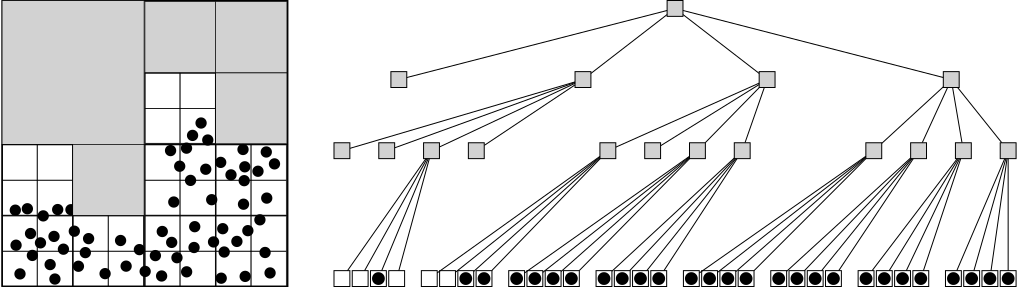
\includegraphics[width=\textwidth]{octree}
  \label{fig:octree}
  \caption[Funktionsweise eines Octrees]{Quadtree (2d-Äquivalent des Octrees) zur Veranschaulichung der Funktionsweise eines Octrees:
    Räumliche Unterteilung und deren die Baum-Darstellung.
    Rekursive Zerlegung der interessanten Zellen bis zur gewünschten Auflösung in Ebene 4, dann zellweises Binning der Atome.
  }
\end{figure}

\begin{algorithm}
  \begin{algorithmic}
%    \Input $root$ - Stammzelle des Octrees
%    \Input $i[3]$ - globale Adresse der Zielzelle
%    \Input $allocate$ - Ob die Zelle neu erstellt werden soll
    \Result null falls leer, sonst Zielzelle
    \State
    \Function{getcell-octree}{$cell, id, allocate$}
    \State $d \gets $\Call{depth}{root}
    \Comment{Relative Tiefe, an der sich die Zielzellen befinden}
    \If{$d = 0$}
    \State\Return cell
    \EndIf
    \If{not $cell.children$}
    \If{allocate}
    \State $cell.children \gets $new cell[8]
    \Else
    \State \Return null
    \EndIf
    \EndIf
    \State $childid \gets $\Call{bitand}{id[0], $2^{d-1}$}
    + $2\cdot$\Call{bitand}{id[1], $2^{d-1}$}
    + $4\cdot$\Call{bitand}{id[2], $2^{d-1}$}
%    \State \Comment{Indiziert die Subzelle aus der globalen Position}
    \State \Return\Call{getcell-octree}{$cell.children[childid], i, allocate$}
    \EndFunction
  \end{algorithmic}
  \caption[Zell-Addressierung in Octrees]{Rekursive Zell-Addressierung und -Allokierung im Octree: Bei jedem Schritt wird das Problem in 8 Unterzellen geteilt, woraus eine Laufzeit von \BigO{d}$=$\BigO{\log{c}} resultiert}
  \label{algo:octreeadressing}
\end{algorithm}

\todo[inline]{Wars das? Formeln?}

\subsection{k-d-Bäume}

Für Nachbarschafts- und Bereichssuchen wird wegen ihrer hervorragenden Suchkomplexität auf k-d-Bäume zurückgegriffen, die einen kartesischen Raum in orthogonale Zellen mit jeweils einem Atom unterteilen.
Es ergibt sich ein balancierter Binärbaum mit Atomen als Knoten, dessen Haupteigenschaft in impliziter Betrachtung von Abstandsrelationen liegt.
So lassen sich große Bereiche aus einer Abstandssuche oder Bereichssuche ausschließen, sobald ein Atom mit geringerem Abstand gefunden wurde.
Somit lässt sich per binärer Suche das nächste Atom eines beliebigen Punktes in \BigO{\log{n}} finden.
Sucht man $N$ Nächstnachbaratome, lassen sie sich durch Kombination mit einem Heap in \BigO{\log{n}\log{N_r}} finden, was zwar im Vergleich zu Octrees zu höheren asymptotischen Laufzeiten führt, jedoch zu kürzeren realen Laufzeiten führt.
\footnote{Vergleich dazu auch Heapsort vs. Quicksort: Cachingeffekte}
Aktualisierungen von Knoten behandelt man durch Standardalgorithmen wie Baumrotation in \BigO{\log{n}}.

Eine weitere Eigenschaft von k-d-Bäumen ist außerdem, dass sie nicht auf endliche Räume beschränkt sind und zuverlässig beliebig große Systeme beschreiben können.
Durch adaptives Neubalancieren erreicht man dennoch bei typischerweise einseitigem Schichtwachstum die oben erwähnten Suchlaufzeiten auf Kosten der Manipulationseffizienz.

\begin{figure}[bthp]
  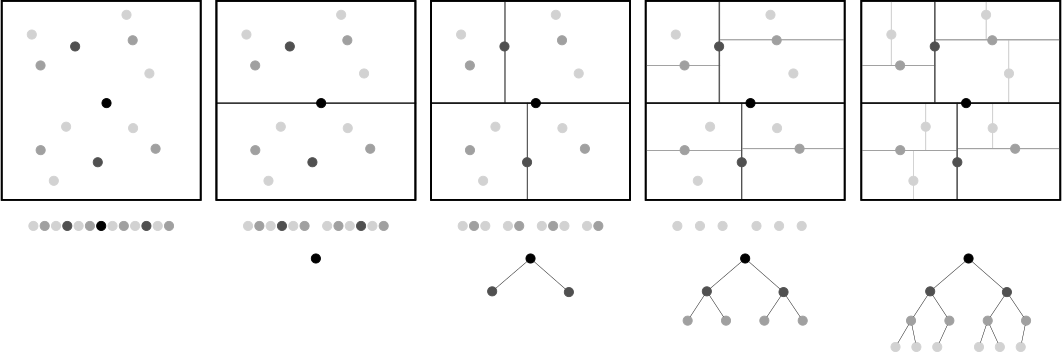
\includegraphics[width=\textwidth]{kdtree-tree}
  \caption[Konstruktion eines k-d-Baumes]{
    Rekursive Konstruktion eines k-d-Baumes: Die Punktmenge wird sortiert, der Median zum Baum hinzugefügt und seine Kinder aus den beiden Teilmengen per k-d-Baum-Konstruktion gewonnen.
    Der gewonnene Suchbaum ist effizient in Speicherplatz und Laufzeit der Suchoperationen.
  }
  \label{fig:kdtree}
\end{figure}

%% \begin{algorithm}
%%   \begin{algorithmic}
%%     \Input $points$ - Liste von Punkten
%%     \Input $k$ - Dimensionalität des Simulationsraumes
%%     \Result Root-Element eines vollständigen KD-Baumes aus diesen Punkten
%%     \State
%%     \Function{construct-kdtree}{$points, dim\gets0$}
%%     \State $n\gets$\Call{length}{points}
%%     \If{$n=0$}
%%     \State \Return null
%%     \Else
%%     \State \Call{sort}{$points, dim$} \Comment{Sortiert $points$ nach pos[$dim$]}
%%     \State $root\gets{}points\left[\lfloor\frac{n}{2}\rfloor\right]$
%%     \State $dim\gets(dim+1)\mod{k}$
%%     \State $root.left \gets$ \Call{construct-kdtree}{$points\left[0:\lfloor\frac{n}{2}\rfloor-1\right], dim$}
%%     \State $root.right \gets$ \Call{construct-kdtree}{$points\left[\lfloor\frac{n}{2}\rfloor+1:n-1\right], dim$}
%%     \State \Return $root$
%%     \EndIf
%%     \EndFunction
%%   \end{algorithmic}
%%   \caption[Konstruktion eines k-d-Baumes]{Rekursive Konstruktion eines k-d-Baumes (naive Implementierung)}
%%   \label{algo:kdtree-construction}
%% \end{algorithm}

Probleme von k-d-Bäumen zeigen sich bei der Suche nach einer Oberfläche einerseits und bei periodischen Räumen andererseits.
Die Oberfläche entlang einer Hauptachse lässt sich per Range Search mit anschließender Minimalsuche entlang der Suchachse effizient ermitteln, möchte man allerdings das Auftreffen eines Precursors mit beliebiger Inklination ermitteln, kann man auf keine optimale Methode zurückgreifen, sondern muss die Range Search auf einen größeren orthogonalen Suchbereich erweitern und darin eine Auswahl treffen.
Zudem führen lokale Aktualisierungen im schlimmsten Fall zur Neubalancierung des gesamten Baumes, wodurch die Betrachtung paralleler verzögerter Aktualisierungen erschwert wird.
Periodische Simulationsräume führen außerdem in der Nähe der Systemgrenze zu identischen Operationen auf periodischen Bildern des Baumes, die bei eventuellen Aktualisierungen ebenso weitreichende Restrukturierungen zur Folge haben.

Aus diesen Gründen lassen sich k-d-Bäume nicht zufriedenstellend im Parsivald-Modell nutzen.

\subsection{Delaunay-Triangulation}\label{datadelaunay}

\begin{figure}[bhpt]
  \centering
  \def\svgwidth{\textwidth}
  \input{img/delaunay.pdf_tex}
  \caption[Delaunay-Triangulation]{Beispiel der Konstruktion einer Delaunay-Triangulation (c) aus einer Punktwolke (a).
    Für jedes Simplex (hier 2d-Simplex, also Dreieck) muss das Delaunay-Kriterium eingehalten werden:
    Es dürfen sich keine weiteren Punkte im Umkreis des Simplices befinden (b).
  }
  \label{fig:delaunay}
\end{figure}

Eine alternative Partitionsmethode findet sich in Triangulationen, die die konvexe Hülle der Punktwolke raumfüllend in nichtüberlappende k-dimensionale Simplexe entsprechend einer weiterhin Delaunay-Kriterium genannten Beziehung zerlegen:
Im Umkreis eines Simplexes befinden sich keine weiteren Punkte aus der Punktwolke.
Damit ergibt sich eine Vielzahl an Eigenschaften, die für verschiedene Problemstellungen zu effizienten Lösungen führen.
So beinhaltet eine Delaunay-Triangulation als Subgraphen den Nächstnachbargraphen, die Alpha-Form und die konvexe Hülle, ist dual zum Voronoi-Diagramm und es lässt sich leicht auf Konnektivität prüfen.


\begin{itemize}
\item Jeder Punkt ist Eckpunkt eines oder mehrerer Simplexe
\item Simplexe überschneiden sich nicht
\item Im Umkreis eines Simplexes befinden sich keine weiteren Punkte
\item Die Vereinigung aller Simplexe ergibt die konvexe Hülle
\item Alpha-Form $\subset$ Delaunay-Triangulation
\item %Ein Punkt teilt sich mit seinem nächsten Nachbarn mindestens einen Simplex \\
  %$\Leftrightarrow$
  Nächstnachbargraph $\subset$ Delaunay-Triangulation
  %% \item Die Delaunay-Triangulation und das Voronoi-Diagramm über die selben Punkte sind dual\\
  %% $\Rightarrow$ Allgemeine Nachbarschaftssuche ist \BigO{k\log k}
\end{itemize}

Delaunay-Triangulationen werden somit für Oberflächenbetrachtungen interessant, da sie über die Alpha-Form, welche durch Auswahl der Punkte aller Simplexe mit Umkreisradien oberhalb einer stoffabhängigen Grenze ermittelt wird und die wahrgenommene Oberfläche eines Systems darstellt.
Somit lassen sich Oberflächenrauheiten, Nanoporen und bei extremen Grenzwerten auch Kristalldefekte bestimmen.
Mit wenig Mehraufwand gegenüber reinen Delaunay-Triangulationen ließen sich somit einerseits Auswertungen bei laufenden Simulationen durchführen und Prozesse gegebenenfalls direkt optimieren, andererseits ist die gesamte Oberfläche zur Simulation von Oberflächenereignissen bekannt und direkt parametrisiert.

\subsubsection{Algorithmen zur Konstruktion einer Delaunay-Triangulation}

Zur Delaunay-Triangulierung aus einer Punktmenge stehen verschiedene Algorithmen zur Verfügung, die auf unterschiedlichen Methoden aufbauen.

\begin{itemize}
\item Flip-basierte Algorithmen (Local Improvement)\\
  Man startet mit einer beliebigen Triangulation, prüft den Umkreis aller Simplexe auf enthaltene Punkte und korrigiert gegebenenfalls per Flip-Algorithmus, der in Abbildung \ref{fig:delaunay-flip} dargestellt ist.
  Diese Algorithmen konvergieren typischerweise in \BigO{n^2} und sind damit vergleichsweise langsam.

\item Scan-Algorithmus (Incremental Construction)\\
  Man konstruiert schrittweise Simplexe, die das Delaunay-Kriterium erfüllen und keine nachträgliche Änderung benötigen.
  Durch viele Vergleiche und Sortierungen varieren typische asymptotische Laufzeiten zwischen \BigO{n\log{n}} und \BigO{n^2}.

\item Einfügungs-Algorithmen (Incremental Insertion)\\
  Man erstellt einen beliebig großen Simplex, der die gesamte Punktmenge beinhaltet, und fügt schrittweise einzelne Punkte in die Triangulation ein.
  Der den eingefügten Punkt umfassende Simplex wird an ihm in mehrere Unter-Simplexe geteilt, auf den und dessen unmittelbare Nachbarn ein Flip-basierter Algorithmus ausgeführt wird.
  Laufzeiten sind typischerweise gering mit \BigO{n\log{n} + n^{\lceil d/2 \rceil}}.

\item Divide-and-Conquer-Algorithmen\\
  Man teilt die Punktmenge in Untermengen, die rekursiv trianguliert und anschließend an ihren Grenzen miteinander zur Zieltriangulation vereinigt werden.
  Hauptproblem ist die Vereinigung der Teiltriangulierungen, die in zwei Dimensionen aufgrund von Ordnungsrelationen entlang der Grenze beinahe trivial, in höheren Dimensionen jedoch mit Problemen verbunden ist.
  Eine mögliche Lösung ist der DeWall-Algorithmus\cite{cignoni_1998}, dessen Verknüpfungsoperation entlang der Grenzen teilperiodischer Räume interessant wird.
  In zwei Dimensionen erreicht man \BigO{n\log{n}}, höhere Dimensionen können per DeWall-Algorithmus mit einer Laufzeit von \BigO{n^{\lceil d/2 \rceil + 1}} behandelt werden, die sich jedoch nur in pathologischen Fällen zeigt.
  Nimmt man annähernde Gleichverteilungen an, konvergiert dieser Algorithmus in drei Dimensionen subquadratisch, man sollte jedoch betrachten, dass er sich gegenüber anderer Konstruktionsalgorithmen durch einfache Parallelisierung sowie der Möglichkeit der Aktualisierung großer Raumbereiche auszeichnet.

\item Höherdimensionale Einbettung\\
  Hier wird die Punktmenge in eine höhere Dimension transformiert, in der deren konvexe Hülle berechnet wird, die dann in den ursprünglichen Raum herunterprojiziert wird und darin eine gültige Delaunay-Triangulation ergibt.
  Dieser Algorithmus ist von rein akademischem Interesse, da Einfügungs-Algorithmen für allgemeine Fälle geringere Laufzeiten ermöglichen.
  Interessant wird diese Methode ebenfalls bei Hinzufügung und Aktualisierung von Punkten.

\end{itemize}

\subsubsection{Flip-Algorithmus}

\begin{figure}[bhpt]
  \captionsetup[subfigure]{singlelinecheck=false}{
    \def\subfigwidth{0.23\textwidth}
    \def\svgwidth{\textwidth}
    \begin{subfigure}[t]{\subfigwidth}
      \includegraphics[width=\textwidth]{delaunay-flip-a}
      \subcaption{Ausgangstriangulation}
      \label{fig:delaunay-flip-a}
    \end{subfigure}
    \hfill
    \begin{subfigure}[t]{\subfigwidth}
      \includegraphics[width=\textwidth]{delaunay-flip-b}
      \subcaption{Vereinigung invalider Simplexe}
      \label{fig:delaunay-flip-b}
    \end{subfigure}
    \hfill
    \begin{subfigure}[t]{\subfigwidth}
      \includegraphics[width=\textwidth]{delaunay-flip-c}
      \subcaption{Aufteilung in neue valide Simplexe}
      \label{fig:delaunay-flip-c}
    \end{subfigure}
    \hfill
    \begin{subfigure}[t]{\subfigwidth}
      \includegraphics[width=\textwidth]{delaunay-flip-d}
      \subcaption{Ergebnis}
      \label{fig:delaunay-flip-d}
    \end{subfigure}
  }
  \caption{
    Flip-Algorithmus: Invalide Simplexe werden aufgelöst und entlang einer neuen Grenze in neue Simplexe überführt.
    Diese Operation läuft in \BigO{k_d\log{k_d}} Prüfungen bei Aktualisierung der Punkte eines Simplexes, mit $k_d$ als oberer Schranke der Zahl der Simplexe eines Punktes.
  }
  \label{fig:delaunay-flip}
\end{figure}

Basis vieler Algorithmen auf Delaunay-Triangulationen basieren auf dem \textbf{Flip-Verfahren} (Abbildung \ref{fig:delaunay-flip}), mit dem unzulässige in zulässige Simplexe überführt werden.
Dabei werden Grenzen zu dem benachbarten Simplex, dessen Punkt innerhalb des Umkreises liegt, aufgelöst und aus den dann verfügbaren Punkten zwei neue Simplexe gebildet.
Im Anschluss ist es häufig notwendig, die neu entstandenen Simplexe sowie die ursprünglichen Nachbarn des zweiten Simplexes auf die gleiche Art zu prüfen.

%% Nachbarschaftssuche nicht notwendig

%% \subsubsection{Nachbarschaftssuche}
%% Für die Nachbarschaftssuche eines Referenzpunktes werden die raumfüllenden Eigenschaften der Triangulation relevant.
%% Der notwendigerweise konvexe, sonst aber beliebige Suchbereich um den Referenzpunkt wird von Simplexen überdeckt, die in direkter oder indirekter Nachbarschaft des Punktes liegen.
%% Somit teilen sich alle Punkte innerhalb des Suchbereiches eine Kante eines Simplexes mit einem anderen Punkt im Suchbereich, sofern der Suchbereich hinreichend groß ist.
%% Ausgehend vom Referenzpunkt sucht man entlang aller Kanten nach Punkten, die innerhalb des Suchbereiches liegen, bis alle potentiellen Punkte überprüft wurden.
%% Diese Vorgehensweise ist in Algorithmus \ref{algo:delaunay-neigbors} ausführlich beschrieben.

%% \begin{algorithm}
%%   \centering
%%   \begin{algorithmic}
%%     \State Result = \{\}
%%     \State Queue = \{ P$_0$ : P$_0 \in$ Volume \}
%%     \While{Queue $\neq \emptyset$}
%%     \State Sei P $\in$ Queue
%%     \State Queue = Queue $\setminus$ \{ P \}
%%     \If{P $\in$ Volume}
%%     \State Result = Result $\cap$ \{ P \}
%%     \State Queue $\cap$ (Neighbors(P) $\setminus$ Result)
%%     \EndIf
%%     \EndWhile
%%   \end{algorithmic}
%%   \caption[Nachbarschaftssuche auf einer Delaunay-Triangulation]{Nachbarschaftssuche auf einer Delaunay-Triangulation.
%%     Ist der Suchraum konvex und hinreichend groß, lässt sich damit effizient nach Nachbarn eines bestimmten Punktes suchen.
%%   }
%%   \label{algo:delaunay-neighbors}
%% \end{algorithm}

\subsubsection{Alpha-Form}

Die Alpha-Form (Abbildung \ref{fig:delaunay-alpha}) beschreibt anschaulich, aus welchen Punkten, Linien und Flächen die Oberfläche einer Punktmenge besteht.
Im Gegensatz zur konvexen Hülle kann sie auch Einschlüsse, Poren und Oberflächenrauheiten je nach Wahl des $\alpha$-Wertes darstellen.
Allgemeine Hüllen von Triangulationen werden dabei als Vereinigung der Menge genau der Flächen gewonnen, die nur einem Simplex zugeordnet sind, so dass man die konvexe Hülle beispielsweise als Hülle einer Delaunay-Triangulation erhält.
%% Abhängig vom Anwendungsfall lassen sie sich als Menge von Punkten, Verbindungslinien oder Flächen ausdrücken.

Für die Konstruktion von Alpha-Formen aus Delaunay-Triangulationen gibt es dabei zwei äquivalente Ansätze:
Einerseits kann man alle Simplexe mit einem Umkreisradius $r_d > \alpha^{-1}$ aus der Delaunay-Triangulation entfernen und die Hülle der so entstandenen Triangulation bilden.
Andererseits kann man alle Simplexe mit einem Umkreisradius $r_d > \alpha^{-1}$ aus der Delaunay-Triangulation auswählen und deren Hülle bilden.
Die Nutzung des $\alpha$ als inversen Parameter ergibt sich hierbei aus weitergehenden Überlegungen, die konvexe Hülle als $\alpha=0$ und Tests mit invertierten Kreisflächen als $\alpha<0$ darzustellen.

Beide Methoden erzeugen dabei leicht unterschiedliche Ergebnisse:
Ansatz 1 garantiert, dass die so entstandenen Oberflächen aus Simplexen aufgebaut sind, also keine einzelnen Punkte oder Dreiecke beinhalten und somit eines oder mehrere Volumen beschreiben.
Ansatz 2 erzeugt in erster Linie die gleiche Oberfläche, erfasst allerdings zusätzlich innerhalb der Auswahl auch einzelne Atome, Verbindungslinien oder Flächen, die keinem Volumen zugeordnet sind und somit im atomistischen Kontext einzelne Atome oder kleine Moleküle darstellen.
Um beim zweiten Ansatz auch Elemente der konvexen Hülle erfassen zu können, wird die Triangulation häufig innerhalb und inklusive der Eckpunkte eines unendlichen virtuellen Simplexes vorgenommen, wie es auch bei einigen Konstruktionsmethoden üblich ist.
Per Konnektivitätsprüfung der Oberflächendreiecke lässt sich zwischen zusammenhängenden Oberflächen, Einschlüssen und eigenständigen Punkten unterscheiden.

In der Anwendung werden Alpha-Oberflächen für die Bestimmung von Rauheiten von Oberflächen oder Volumen poröser Materialien interessant, da sie sich als Punktmengen- beziehungsweise Polygonoperationen gestalten.
Für Simulationen von Oberflächenabscheidungen ließen sich auf diese Weise auch Bedeckungen mit Precursorliganden ermitteln.

\begin{figure}[bhpt]
  \centering
  \captionsetup[subfigure]{singlelinecheck=false}{
    \def\subwidth{0.4\textwidth}
    \def\svgwidth{\textwidth}
    \begin{subfigure}[t]{\subwidth}
      
\includegraphics[width=\textwidth]{delaunay-alpha-a}
      \subcaption{Delaunay Triangulation einer beliebigen Punktmenge}
      \label{fig:delaunay-alpha-a}
    \end{subfigure}
    \hfill
    \begin{subfigure}[t]{\subwidth}
      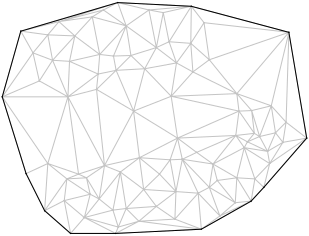
\includegraphics[width=\textwidth]{delaunay-alpha-b}
      \subcaption{Konvexe Hülle: Hülle der Triangulation}
      \label{fig:delaunay-alpha-b}
    \end{subfigure}
  }
  \vspace{2em}
  \captionsetup[subfigure]{singlelinecheck=false}{
    \def\subwidth{0.4\textwidth}
    \def\svgwidth{\textwidth}
    \begin{subfigure}[t]{\subwidth}
      \includegraphics[width=\textwidth]{delaunay-alpha-c}
      \subcaption{Alpha-Form: Hülle nach Entfernung von Simplexen mit $r_d > \alpha$}
      \label{fig:delaunay-alpha-c}
    \end{subfigure}
    \hfill
    \begin{subfigure}[t]{\subwidth}
      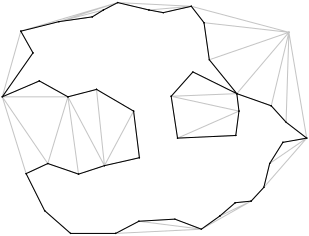
\includegraphics[width=\textwidth]{delaunay-alpha-d}
      \subcaption{Alpha-Form: Hülle nach Entfernung von Simplexen mit $r_d < \alpha$ (nur innen)}
      \label{fig:delaunay-alpha-c}
    \end{subfigure}
  }
  \caption[Methoden zur Bestimmung der Oberfläche per Delaunay-Triangulation]{Verschiedene Methoden zur Bestimmung der Oberfläche per Delaunay-Triangulation. Man beachte, dass die in (d) genutzte Methode den Ausreißer-Punkt oben rechts mit trianguliert, jedoch nicht zur Oberfläche zählt, da für keinen seiner Simplexe $r_d < \alpha$ gilt}
  \label{fig:delaunay-alpha}
\end{figure}

